\section{Results and Analysis}

\begin{frame}
\frametitle{Comparison of Insertion Sort and Quick Sort}
  \framesubtitle{Execution Time for Different Data Sizes}
\begin{columns}
    \begin{column}{0.3\textwidth}
      \centering
      \textbf{Execution time for Insertion Sort and Quick Sort in C++ Language}

    \end{column}
    \begin{column}{0.7\textwidth}
       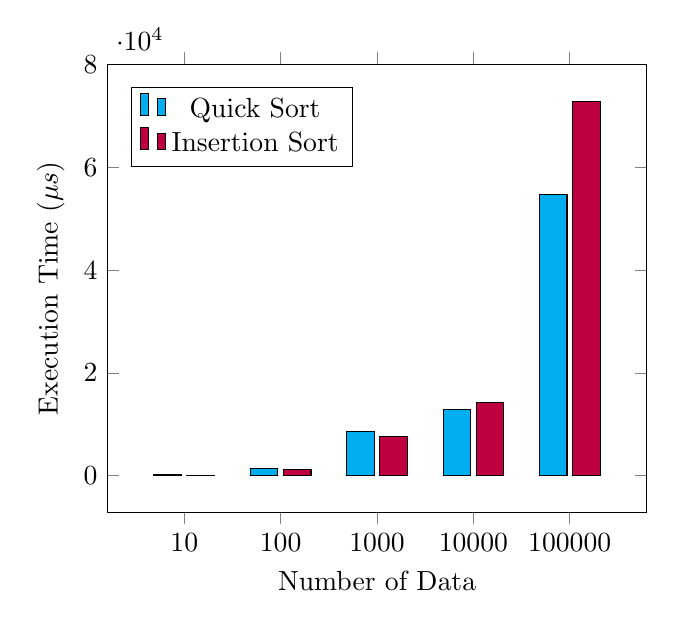
\begin{tikzpicture}
    \begin{axis}[
      ybar,
      bar width=0.35cm,
      xlabel={Number of Data},
      ylabel={Execution Time ($ \mu s $)},
      symbolic x coords={10, 100, 1000, 10000, 100000},
      xtick=data,
      legend style={at={(0.25,0.95)},anchor=north},
      enlarge x limits={0.2},
    ]

    \addplot[fill = cyan] coordinates {(10,138) (100,1458) (1000,8585) (10000,12917) (100000,54659)};
      \addlegendentry{Quick Sort}
      \addplot[fill = purple] coordinates {(10,85) (100,1257) (1000,7580) (10000,14312) (100000,72819)};
      \addlegendentry{Insertion Sort}

    \end{axis}

  \end{tikzpicture}
    \end{column}
  \end{columns}
\end{frame}

\begin{frame}
\frametitle{Comparison of Insertion Sort and Quick Sort}
  \framesubtitle{Execution Time for Different Data Sizes}
\begin{columns}
    \begin{column}{0.3\textwidth}
      \centering
      \textbf{Execution time for Insertion Sort and Quick Sort in Python Language}

    \end{column}
    \begin{column}{0.7\textwidth}
       \begin{tikzpicture}
    \begin{axis}[
      ybar,
      bar width=0.35cm,
      xlabel={Number of Data},
      ylabel={Execution Time ($ \mu s $)},
      symbolic x coords={10, 100, 1000, 10000, 100000},
      xtick=data,
      legend style={at={(0.25,0.95)},anchor=north},
      enlarge x limits={0.2},
    ]

    \addplot[fill = statalegreen] coordinates {(10,614) (100,7805) (1000,35644) (10000,46016) (100000,187876)};
      \addlegendentry{Quick Sort}
      \addplot[fill = blue] coordinates {(10,474) (100,5697) (1000,44289) (10000,66598) (100000,256741)};
      \addlegendentry{Insertion Sort}
    \end{axis}

  \end{tikzpicture}
    \end{column}
  \end{columns}
\end{frame}




\begin{frame}
  \frametitle{Theoretical Background}
  \framesubtitle{Time and Space Complexity}

  \textbf{Insertion Sort}
  \begin{itemize}
    \item Time Complexity:
      \begin{itemize}
        \item Worst Case: \(O(N^2)\)
        \item Best Case: \(O(N)\)
      \end{itemize}
    \item Space Complexity: \(O(1)\)
  \end{itemize}

  \textbf{Quick Sort}
  \begin{itemize}
    \item Time Complexity:
      \begin{itemize}
        \item Average: \(O(N \log N)\)
        \item Worst Case: \(O(N^2)\) (e.g., when the array is sorted in reverse)
      \end{itemize}
    \item Space Complexity: \(O(\log N)\)
  \end{itemize}
\end{frame}

\begin{frame}
  \frametitle{Practical Observations}
  \framesubtitle{Performance on Different Data Sizes}

  For smaller data (e.g., 100), Insertion Sort outperforms Quick Sort. For larger datasets (e.g., 100,000), Quick Sort performs better.

  \vspace{1em}

  \textbf{Sorted Data Set:}
  \begin{itemize}
    \item Insertion Sort outperforms Quick Sort.
    \item True for any dataset size.
  \end{itemize}
\end{frame}

\begin{frame}
  \frametitle{Language Dependency}
  \framesubtitle{Python, Java, and C++}

  Python takes more time to implement despite following theoretical aspects. Python's dynamic typing may contribute to this. Java and C++, statically typed languages, show slightly better execution speed.

  \vspace{1em}

  \textbf{Recommendation:}
  \begin{itemize}
    \item Python is easier to read but slower.
    \item For efficiency, use C++ or Java.
  \end{itemize}
  
\end{frame}

